\section{ フォトグラフ}
\large{

そこには まだ\ruby{虹}{にじ}があるの?

\ruby{花}{はな}たちが\ruby{育}{そだ}ってゆくの?

We laughed them all

\ruby{気}{き}づかない\ruby{程}{ほど}\ruby{若}{わか}くないし

\ruby{理解}{りかい}できない\ruby{程}{ほど}

\ruby{純真}{じゅんしん}でもない\ruby{天使}{てんし}たち

\ruby{本当}{ほんとう}は\ruby{怖}{こわ}くて \ruby{本当}{ほんとう}は\ruby{弱虫}{よわむし}

\ruby{帰}{かえ}る\ruby{家}{いえ}を\ruby{探}{さが}してる
\\

そばに\ruby{居}{い}るだけで それだけでよかった

\ruby{フォトグラフ}{photograph} \ruby{明日}{あした}が\ruby{見}{み}えなくても

ほら \ruby{君}{きみ}が\ruby{揺}{ゆ}れてる
\\

\ruby{窓辺}{まどべ}に\ruby{並}{なら}べかけた\ruby{植物}{はな}の\ruby{傍}{そば}に

ひとり\ruby{腰}{こし}かけた

There's no time at all

\ruby{思}{おも}い\ruby{入}{い}れが\ruby{強}{つよ}すぎると

\ruby{次}{つぎ}に\ruby{起}{お}こることが\ruby{噓}{うそ}のよう

もう\ruby{何年}{なんねん}ぐらい\ruby{過}{た}ったのだろう

すべてが\ruby{現実}{げんじつ} すべてがまぼろし

\ruby{帰}{かえ}る\ruby{道}{みち}を\ruby{探}{さが}してる
\\

\ruby{言葉}{ことば}はいらなかった

「\ruby{愛}{あい}してる」の\ruby{サイン}{sign}だけで

\ruby{フォトグラフ}{photograph} \ruby{砂}{すな}に\ruby{足跡}{あしあと}つけて

ほら \ruby{君}{きみ}が\ruby{笑}{わら}ってる
\\

そばに\ruby{居}{い}るだけで それだけでよかった

\ruby{瞳}{ひとみ}を\ruby{輝}{かがや}かせ \ruby{夢中}{むちゅう}になるクセ

\ruby{今}{いま}も \ruby{変}{か}わらずにいて

ほら \ruby{君}{きみ}が\ruby{愛}{いと}しい

}

{ \ }

{ \ }

{ \ }

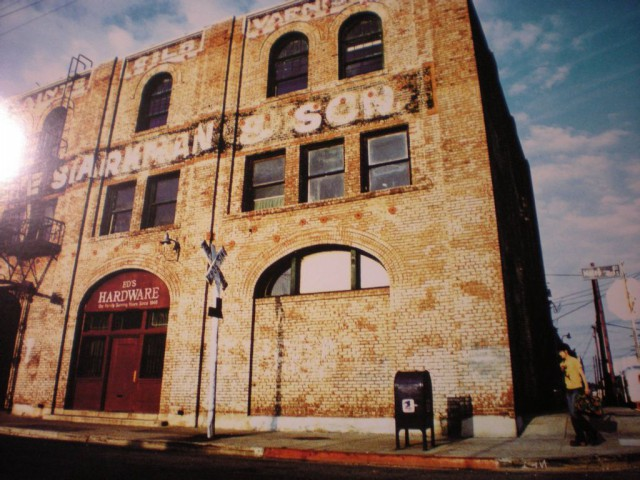
\includegraphics[width=0.9\textwidth]{P6.jpg}